\documentclass[a4paper, 12pt]{report}

%%%%%%%%%%%%
% Packages %
%%%%%%%%%%%%

\usepackage[english]{babel}
\usepackage[noheader]{packages/sleek}
\usepackage{packages/sleek-title}
\usepackage{packages/sleek-theorems}
\usepackage{packages/sleek-listings}
\usepackage{titlesec}
\usepackage{lipsum}
\usepackage{biblatex}
\usepackage{mathtools}
\usepackage{amsmath}
\usepackage{algorithm}
\usepackage{algcompatible}
\usepackage{algpseudocode} 
\usepackage{tikz}
\usepackage{caption}
\usepackage{subcaption}
\usepackage{pgfplots}
\usepackage{indentfirst}
\usepackage{gensymb}

\titleformat{\chapter}[display]
  {\normalfont\bfseries}{}{0pt}{\Large}
  
  \newenvironment{conditions}
  {\par\vspace{\abovedisplayskip}\noindent\begin{tabular}{>{$}l<{$} @{${}={}$} l}}
  {\end{tabular}\par\vspace{\belowdisplayskip}}
  
 \nocite{*}

%%%%%%%%%%%%%%
% Title-page %
%%%%%%%%%%%%%%

\logo{./img/feup.png}
\institute{Faculty Of Engineering, University Of Porto}
\faculty{Informatics and Computing Engineering Department}
\subtitle{Algorithm Design and Analysis}
%\department{Department of Anything but Psychology}
\title{Looking for a parking place}
\author{\textit{Authors}\\André \textsc{Moreira}, 201904721
        \\Nuno \textsc{Alves}, 201908250
        \\Nuno \textsc{Costa}, 201906272}
%\supervisor{Linus \textsc{Torvalds}}
%\context{Well, I was bored...}
\date{\today}

%%%%%%%%%%%%%%%%
% Bibliography %
%%%%%%%%%%%%%%%%

\addbibresource{./resources/bib/references.bib}

%%%%%%%%%%
% Others %
%%%%%%%%%%

\lstdefinestyle{latex}{
    language=TeX,
    style=default,
    %%%%%
    commentstyle=\ForestGreen,
    keywordstyle=\TrueBlue,
    stringstyle=\VeronicaPurple,
    emphstyle=\TrueBlue,
    %%%%%
    emph={LaTeX, usepackage, textit, textbf, textsc}
}
\renewcommand{\baselinestretch}{1.1} 
\setlength{\parskip}{0.5em}
\setlength{\parindent}{1em}

\FrameTBStyle{latex}

\def\tbs{\textbackslash}

%%%%%%%%%%%%
% Document %
%%%%%%%%%%%%

\pgfplotsset{compat=1.17}
\begin{document}
    \maketitle
    
    \romantableofcontents
    
    \chapter{Introduction} \label{intro}
    
    Parking management in a big city can be quite challenging. Efficiently managing availability, time and cost is a tough task, even when all the information is gathered.
    
    Furthermore, people don't always know where the parking spots are located and which ones are available, which may result in congested city traffic, parking allocation inefficiency or time wasted in the inevitable task of finding a parking place.
    
    The problem that will be analysed in this project derives from the Travelling Salesman Problem. Given the origin and destination locations, a suitable parking spot, as well as the path to it that goes through all chosen points of interest, should be found. For this, the chosen solution must account for a set of variables and restrictions. The chosen parking spot must be available, close to the destination location - within reasonable walking distance -, should be as cheap as possible and the path's distance must also be as short as possible.
    
    However, meeting all these conditions and obtaining the best solution possible can become time costly, especially as the problem's size grows. Time complexity is an important measure to calculate the viability of an algorithm and should be also accounted for.
    
    With all of this in mind, the following report seeks to solve this problem and all of its intricacies, aiming for a real-life solution to the problem.
    
    \newpage
    
    
    \chapter{Problem Definition} \label{pdef}
    
    In this chapter the problem is defined in terms of input data, output data, its constraints and the objective function. 
    
    \section{Input Data} \label{idata}
    
    All the needed information to compute a solution for the problem is defined below. It should be noted that the following structures represent the input data needed - additional parameters may be added to the structures defined below for the algorithms that need them.
    
    \subsection{Definition}
    
    \begin{enumerate}
        \item The map should be represented by a directed graph $G = (N,E)$, where
        \begin{enumerate}
            \item $N$ is the set of nodes of the graph.
            \item $E$ is the set of edges of the graph (where the edges represent any given connection between two nodes, being it a street, a highway, etc.).
        \end{enumerate}
    
        \item $N_{k} \in N$, $1 \leqslant k \leqslant |N|$ is a node of the graph represented by a tuple $N_k = (la, lo, A, P_{info})$ where
        \begin{enumerate}
            \item $la(N_k)$ is the latitude of the node.
            \item $lo(N_k)$ is the longitude of the node. 
            \item $A(N_k)$ is the set containing edges connected to the node, such that $A \subseteq E$.
            \item $P_{info}(N_k)$ is the parking information associated to that node.
            \begin{enumerate}
                \item If N is a parking lot, $P_{info}(N_k)$ represents a parking lot $P_k = (c,c_{max},f) \in P$, $1 \leqslant k \leqslant |P|$  where
                \begin{enumerate}
                    \item $c(P_k)$ is its current capacity.
                    \item $c_{max}(P_k)$ is its maximum capacity.
                    \item $f(P_k) = f(t,o)$ is the parking fee function, which can vary both according to the parking time $t_k \in t_{parking}$ and the occupancy rate $o = \frac{c}{c_{max}}$.
                \end{enumerate}
                \item If N is not a parking lot, $P_{info}(N_k) = (r_{parking})$, where
                \begin{enumerate}
                    \item $r_{parking}$ is a boolean that defines whether or not this node requires nearby parking, in case of it being a POI for the user.
                \end{enumerate}
            \end{enumerate}
        \end{enumerate}
        
        \item $E_{k} \in E$, $1 \leqslant k \leqslant |E|$ is an edge of the graph represented by a tuple $E_k = (N_{origin}, N_{destination}, w)$ where
        \begin{enumerate}
            \item $N_{origin}(E_k) \in N$ is the origin node of the edge.
            \item $N_{destination}(E_k) \in N$ is the destination node of the edge.
            \item $w(E_k)$ is the weight of the edge which constitutes its travel distance.
        \end{enumerate}
    
        \item $O$ is the origin node, $O \in N$.
        \item $D$ is the destination node, $D \in N$.
        \item $POI$ are the nodes/points of interest which the traveler must visit before reaching node $D$, $POI \subseteq N$.
        \item $t_{parking}$ is the array with the parking times of each POI/Destination.
        \item $d_{threshold}$ is the distance the user is willing to walk at most.
    \end{enumerate}
    
    \subsection{Constraints}
    
    \begin{enumerate}
        \item $\forall \: N_k \in N : $
        \begin{enumerate}
            \item $ \; -90\degree \leqslant la(N_k) \leqslant 90\degree $
            \item $ \; -180\degree \leqslant lo(N_k) \leqslant 180\degree$
        \end{enumerate}
        \item $\forall \: N_k \in N, \exists \: E_k \in E : N_{origin}(E_k) = N_k \lor  N_{destination}(E_k) = N_k $
        \item $\forall \: E_k \in E : w(E_k) > 0$ 
        \item $\forall \: P_{k} \in P : \{P_k = P_{info}(N_k)$ where $N_k$ is a parking lot\}, 
        \begin{enumerate}
            \item $ \; c_{max}(P_k) > 0 \;$
            \item $\; 0 \leqslant c(P_k) \leqslant  c_{max}(P_k) \;$
            \item $ \forall \: t \geqslant 0: f(P_k)(t,o) \geqslant 0$
        \end{enumerate}
        \item $O \neq D$
        \item $\forall \: t_k \in t_{parking}: \: t_k > 0$
        \item $|t_{parking}| = |POI| + 1$, which means that every park chosen must have a parking time associated to it (for each POI and destination).
        \item $d_{threshold}$ > 0.
    \end{enumerate}
    
    \pagebreak

    \section{Output Data} \label{odata}
    
    The output of a solution is described below.
    
    \subsection{Definitions}
    
    \begin{enumerate}
        \item The ordered list of paths $S$ that, for each $S_k$, $1 \leqslant k \leqslant |POI|+1$, $S_k = (S^v, S^f)$, where
        \begin{enumerate}
            \item $S^v$ is the ordered list of travelled edges that form the solution path from the origin/last POI node to the parking node $k$ of the POI/destination.
            \item $S^f$ is the ordered list of travelled edges that form the solution path from the parking node to the respective POI/destination node.
        \end{enumerate}
        \item A simplified graph $G_s = (N_s,E_s)$ containing only the nodes and edges that are present in the solution paths $S$, where $N_s \in N \land E_s \in E$.
        \item The chosen parking lots array $P_{chosen} \subseteq N$.
        \item Distance taken by vehicle $ \displaystyle d_{v} = \sum_{i=1}^{|S|}\sum_{k=1}^{|S^v(S_i)|} w_k(S^v(S_i))$.
        \item Distance taken by foot $ \displaystyle d_{f} = \sum_{i=1}^{|S|}\sum_{k=1}^{|S^f(S_i)|} w_k(S^f(S_i))$.
        \item The total price of the parking $p$ given by the function $f(P_{k}) = f(t,o)$ for each parking such that $ \displaystyle p = \sum_{k=1}^{|P_{chosen}|} f(t_k, \frac{c(P_{k} )}{c_{max}(P_{k})})$.
    \end{enumerate}

    \subsection{Constraints}
    \begin{enumerate}
        \item Travelled edges $S^w$
        \begin{enumerate}
            \item The first edge $E_{0}$ of the travelled edges list, $N_{origin}(E_{0})$ must be node $O$.
            \item The last edge $E_{last}$ of the travelled edges list, $N_{origin}(E_{last})$ must be node $P_{chosen}$.
        \end{enumerate}
        \item Travelled edges $S^f$
        \begin{enumerate}
            \item The first edge $E_{0}$ of the travelled edges list, $N_{origin}(E_{0})$ must be node $P_{chosen}$.
            \item The last edge $E_{last}$ of the travelled edges list, $N_{origin}(E_{last})$ must be node $D$.
        \end{enumerate} 
        \item Distance traveled by foot $d_f \geqslant 0$
        \item Distance traveled by vehicle $d_v \geqslant 0$
    
    \end{enumerate}
    
    \pagebreak
    
    \section{Objective Function} \label{ofunc}

    The problem is, in fact, complex. Taking a bottom-up approach on it, one can break it up into 3 core ideas (and 3 distinct objective functions). 
    
    Firstly, an available parking lot near the destination node which minimizes both distances and cost should be found. For that, we can define a function such that:
    
    \begin{equation}
        cost_1(d_f, p) = k_f \times d_f + k_p \times p
    \end{equation}
    where:
    \begin{conditions}
        d_f     &  the distance travelled by foot \\
        p    &  the parking price \\   
        k_f  &  the foot travel distance importance coefficient  \\
        k_p       &  the parking price importance coefficient  \\
    \end{conditions}
    
    The intention is to minimize the cost. As such, the objective function should be $min(cost_1(d_f, p))$. However, it must be noted that this minimum is dynamic - it may very well vary according to the user preferences, or in other words, according to the foot travel distance and price importance coefficients. This function will be 0 if $r_{parking}$ is true for the destination node.
    
    Secondly, the path between the chosen parking lot and the origin should be defined. A cost function for that problem can be defined as:
    
    \begin{equation}
        cost_2(d_v) = d_v
    \end{equation}
    where:
    \begin{conditions}
        d_v     &  the distance travelled by vehicle to the parking lot (or destination if $r_{parking}$ is true)\\
    \end{conditions}
    
    As explained above, the intention is to minimize the cost, which means that the objective function is also defined by $min(cost_2(d_v))$. This can be simplified to $min(d_v)$.
    
    Lastly, we need to join both this approaches and apply them to each origin-POI, POI-POI or POI-destination (origin-destination if no POI exist) path. There's two ways to look at the problem given: either the user already gives an order to search each POI towards the destination node, or the application must be capable of choosing a fitting order (as it must pass through all of them).
    
    If the first situation is at hand, the problem is reduced to applying the first two objective functions to each pair. 
    
    However, that may not be the case. As such, a third objective function must be defined. Since calculating the overall minimum distance for a TSP-like problem would be extremely costly, a shift in perspective must be made. As such, one might simply consider the POIs given, the origin and the destination nodes as one smaller graph, where its edges are defined by the distance between them on the map. With that smaller graph, calculating a TSP-like problem seems feasible. As such, defining $d_{tsp}$ as the distance in that TSP-like sub problem, the third and final objective function can be defined as:
    
    \begin{equation}
        cost_3(d_{tsp}) = d_{tsp}
    \end{equation}
    where:
    \begin{conditions}
        d_{tsp}     &  the total path length of the tour of all nodes of the smaller graph \\
    \end{conditions}
    
    As before, the intention is still to minimize the cost, which leads to the third and final objective function being $min(cost_3(d_{tsp})) = min(d_{tsp})$.
    
    To conclude, the solution must, as such, minimize the first two functions for each pair on the minimized tour defined by the third objective function \footnotemark.
    
    \footnotetext{It should be clear, however, that these functions should be minimized in reasonable running time, which may not lead to the absolute minimum value, but a reasonable near-minimum value instead.}
    
        
    \chapter{Prospective Solution} \label{prosol}
    
    \section{Algorithm Overview and Analysis} \label{analysis}
    
    Due to the nature of this problem, it can be divided into three parts (even though they are not independent), as explained before.
    
    Firstly, one can try to find available parking spots within a reasonable distance of the destination node using a Single Source Shortest Path (SSSP) algorithm. From those found parking spots, a cost evaluation occurs, selecting only one.
    
    Secondly, having the selected parking spot defined, a simple Shortest Path algorithm can be used to find the shortest path between that and the origin node. With that path defined, the solution for the sub-path of the total tour is found. As such, this solution must be applied to all sub-paths of the tour, which is defined either by input or by using a TSP solving algorithm. When all sub-paths are solved, the complete solution is finally defined.
    
    However, it is important to firstly check that the graph given is connected, so that it is assured that a solution can be found.
    
    \subsection{Verifying Graph's Connectivity}
    
    For this solution, it is important that the given graph is strongly connected. In fact, a weakly connected graph would not be enough for the purposes of this problem since it would be possible to select a node that had no path to another selected node. Even if the given graph was unilaterally connected, it wouldn't be enough since the user should have the liberty to travel the opposite direction. As such, a strongly connected graph, which has a path between any pair of nodes (u,v), both from u to v and from v to u, must be given as input.
    
    To verify this condition, a pre-processing algorithm must be run on the graph.
    
    \subsubsection{Strongly Connected Components}
    
    A SSC (short for Strongly Connected Component) is defined as a graph's cycle in which any node can reach any other node in the same SSC.
    
    As explained previously, we must guarantee that the graph is strongly connected. A smart way to do that is to assure that the graph has one and only one SSC. To do this, we can use a SSC algorithm.
    
    There are several algorithms for this purpose, such as the Kosaraju's algorithm and Path-Based strong component algorithm, but we'll focus on the Tarjan's algorithm, due to its $O(|V|+|E|)$ linear time complexity.
    
    \subsubsection{Tarjan's Algorithm}
    
    To understand Tarjan's algorithm, one must first understand the concept of \textbf{low-link values}. A low-link value of a node is the smallest node ID reachable when doing a Depth First Search algorithm from that same node (including itself).
    
    After calculating each node's low-link, it is possible to infer what SSC exist in a graph, since every node in a given SSC will have the same low-link value.
    
    However, this might not be true for every case. This low-link calculation for each node is highly dependent on the Depth First Search algorithm. Diferent traversals will most likely result in diferent results, which can't be true since an unchanged graph should still have the same SSC, no matter the traversal \cite{tarjan}.
    
    To fix this flaw, the Tarjan's algorithm uses what is called the \textbf{stack invariant}. This invariant keeps the valid nodes from which to update low-link values from. As such, nodes are added when they are first encountered and removed when a new SCC is found. With this, the SCC aren't 'contaminated' by other SCC upon the Depth First Search since it is possible to check whether or not the node we're currently comparing to belongs to an already closed SCC (that is, if it isn't on the stack).
    
    The pseudo-code for this algorithm can be defined as follows:
    
    \begin{algorithm}[H]
    	\caption{Tarjan's Algorithm Adaptation} 
	    \begin{algorithmic}[1]
	    \State $sccs \leftarrow 0$
	    \State $currentID \leftarrow 0$
	    \State $stack \leftarrow emptystack()$
	    \State
	    \For{$node \in N$}
	        \State $visited(node) \leftarrow false$
	    \EndFor
	    \For{$node \in N$}
	        \If{not $visited(node)$}
	            \State $dfs(node)$
	        \EndIf
	    \EndFor
		\State \textbf{return} $sccs$ equals $1$
	    \end{algorithmic} 
    \end{algorithm}
    \begin{algorithm}[H]
    	\caption{DFS function}
    	\begin{algorithmic}[1]
	        \State $push(stack, node)$
	        \State $id(node) \leftarrow currentID$
	        \State $lowlink(node) \leftarrow currentID$
	        \State $currentId \leftarrow currentID + 1$
	        \State
	        \For{\textbf{each} $adj \in adj(node)$}
	            \If{not $visited(adj)$}
	                \State $dfs(adj)$
	            \EndIf
	            \If{$adj \in stack$}
	                \State $lowlink(adj) \leftarrow min(lowlink(adj), lowlink(node))$
	            \EndIf
	        \EndFor
	        
	        \State
	        \If{$id(node)$ equals $lowlink(node)$}
	            \While{$pop(stack)$ differs from $node$}
	            \EndWhile
	            \State $sccs \leftarrow sccs + 1$
	        \EndIf
	    \end{algorithmic} 
    \end{algorithm}

        
    With the return value of the previously shown function, it is possible to confirm whether or not the graph is strongly connected. It must be noted, however, that this algorithm opens up possibilities for the solution: if the graph given by input is not strongly connected, but if the nodes given as Origin, points of interest and Destination by the user belong to the same SCC, the algorithm can still run normally (assuming that the SCC has parking spots, which is problem that may be detected later on). This will be taken into consideration upon the implementation.
    
    \subsection{Selecting the best parking spot}  \label{selectpark}
    
    As mentioned, an SSSP algorithm must be used for this part of the solution. For that, a Dijkstra Shortest Path algorithm was chosen (with a time complexity of $O(|E| + |V|log(|V|))$ - using a priority queue).
    
    In order to fulfill the needs of the problem at hand, the algorithm must be modified. As previously mentioned, the user must set a threshold that defines the maximum distance he's willing to walk. The use of a priority queue makes it easier to know when that threshold was surpassed (by definition, we will work with a strictly increasing distance between the source node and current node). 
    
    However, setting only one threshold might not be correct. In a less crowded place, one might find a lot of parking spots in just under 300 meters of the destination, while in some other places with great turnout, there might be fewer available spots throughout a much greater area. As such, to better solve these cases, two thresholds were set, according to the user's max threshold choice.
    
    The following algorithm pseudo-code solves the presented problem.
    
    \begin{algorithm}[H]
    	\caption{Dijkstra Adaptation} 
	    \begin{algorithmic}[1]
		\For {\textbf{each} $vertex \in V $}
		    \State $dist(vertex) \leftarrow \infty$
		    \State $prev(vertex) \leftarrow nil$
		    \State $visited(vertex) \leftarrow false$
		\EndFor
		\State $dist(origin) \leftarrow 0$
		\State $pq \leftarrow makequeue()$
		\State $push(pq, origin)$
		\State
		\State $parks \leftarrow \{\}$
		\State $currdist \leftarrow 0$
		\State $threshold1() \leftarrow $ $return$ $currdist < max1$
		\State $threshold2() \leftarrow $ $return$ $size(parks) < minparks$ $and$ $currdist < max2$
		\State
		
		\While {$pq$ is not empty $and$ ($threshold1()$ $or$ $threshold2())$}
		    \State $current \leftarrow popmin(pq)$
		    \State $currdist \leftarrow dist(current)$
		    \State $visited(current) \leftarrow true$
		    \If{$current$ is parking and not $c(current) = c_{max}(current)$}
		        \State $insert(parks, current)$
		    \EndIf
		    \For{\textbf{each} $edge \in adj(current)$}
		        \State $to \leftarrow to(edge)$
		        \If {$dist(to) > dist(current) + weight(edge)$}
		            \State $dist(to) \leftarrow dist(current) + weight(edge)$
		            \State $prev(to) \leftarrow current$
		            \If {$not$ $visited(current)$}
		                \State $push(pq, to)$
		            \Else
		                \State $decreasekey(pq, to)$
		            \EndIf
		        \EndIf
		    \EndFor
		\EndWhile
		
		\State \textbf{return} $parks$
	    \end{algorithmic} 
    \end{algorithm}
    
    \pagebreak
    
    With the surrounding parks selected, it is key to filter them down. This filter takes into account the distance from the destination node and the price it will charge the user. The distance from the origin shouldn't be a part of this filter: in fact, if a parking spot farther from the origin node is chosen, it means its walking distance to the destination node and price were lower than its counterparts, and the relatively small distance difference (because of the set threshold) shouldn't be accounted for. 
    
    In fact, more than one could be chosen, but this adaptation only makes sense if, in fact, an unpredicted inefficiency on the cost evaluation occurs. In theory, the best parking spot on this phase should still be the best in the following, since the path to it does not impact this decision.
    
    After the applied filter and the chosen parks selected, the algorithm can now proceed to the second part.
    
    \subsection{Shortest path to parking spot} \label{selectpath}
    
    With a best park selected, we can now apply a Shortest Path algorithm to select the best (or an approximation of the best) path from the origin node to that parking spot. For that, the A* algorithm was chosen (an adaptation of Dijkstra's with a heuristic to improve time complexity).
    
    \subsubsection{A* Heuristic Definition} \label{aheuristic}
    
    Since the origin and destination nodes are known, we can define a total distance approximation function $f(node)$, which is defined as
    \begin{equation}
        f(node) = g(node) + h(node)
    \end{equation}
    where:
    \begin{conditions}
        g(node) & the distance from the origin node to the current node \\
        h(node) & an approximation of the distance from the current node to the destination node \\
    \end{conditions}
    
    This approximation distance can be calculated in one of many ways. An easy way to do that would be to consider the remaining distance to the destination node to be the straight line that connects the current node and the destination node. In fact, choosing this distance will make A* always achieve the best solution possible, since it is never an overestimating heuristic of the real remaining distance (as proven in \cite{heuristics}\cite{adaixo}, it is an \textit{admissable} heuristic). However, to make a straight line length calculation, one must use the square root operation, which may not be as efficient. As such, one can use the Manhattan distance, which can be an overestimation of the result in this problem (since it is not a grid map, the user can in fact travel in the shortest diagonal between the two points), and may in fact not lead to the most optimal solution.
    
    With this in mind, it possible to define several distance functions. Since we're given (latitude, longitude) pairs for each node, and the calculation of geodesic distances with the Haversine or Great-circle distance functions is not properly efficient, a variation was found. As such, the straight line distance function can be defined as ($d_{meridian}$ and $d_{equator}$ explained in \cite{distance}):
    
    
    \begin{algorithm}[H]
    	\caption{Distance Function - Haversine variation} 
	    \begin{algorithmic}[1]
		\State $dx = d_{meridian} \frac{|lat_1 - lat_2|}{180}$
		\State $dy = d_{equator} \frac{|lng_1 - lng_2|}{180} cos(\frac{lat1 + lat2}{2})$
        \State $\textbf{return}$ $\sqrt{dx^2 + dy^2}$
	    \end{algorithmic} 
	\end{algorithm}
    As mentioned previously, this could be adapted to use a Manhattan distance, where the use of the square root is ignored, and the sum of the x and y variations is returned instead.
    
    \begin{algorithm}
    	\caption{Distance Function - Haversine variation with Manhattan adaptation} 
	    \begin{algorithmic}[1]
		\State $dx = d_{meridian} \frac{|lat_1 - lat_2|}{180}$
		\State $dy = d_{equator} \frac{|lng_1 - lng_2|}{180} cos(\frac{lat1 + lat2}{2})$
        \State $\textbf{return}$ $dx + dy$
	    \end{algorithmic} 
	\end{algorithm}
    
    It must also be noted that if given grid coordinates, both of this functions can be adapted to be more efficient. With that, the cosine could be ignored and a simple Euclidean distance or, for even more efficiency, a simple Manhattan distance could be calculated.
    
    \subsubsection{A* implementation}
    
    With the heuristic defined, it is now possible to define the algorithm implementation. It must be noted that the implementation which will be described here is a simple A* approach for the problem at hand. Other performance enhancers, such as the bidirectional A* approach, Weighted A* approach or the use of Fibonacci Heaps can and will be taken into consideration in the implementation of the solution.

    \begin{algorithm}[H]
    	\caption{A* algorithm} 
	    \begin{algorithmic}[1]
		\For {\textbf{each} $vertex \in V $}
		    \State $dist(vertex) \leftarrow \infty$
		    \State $prev(vertex) \leftarrow nil$
		\EndFor

		\State $dist(origin) \leftarrow 0$
		\State $pq \leftarrow makequeue()$
		\State $f_{node} \leftarrow dist(origin) + h_{distance}(origin, destination)$
		\State $push(pq, origin, f_{node})$ 
		\algstore{part1}
		\end{algorithmic}
	\end{algorithm}
	
	\pagebreak
	\begin{algorithm}[H]
	    \begin{algorithmic}[1]
	    \algrestore{part1}
		\While {$pq$ is not empty}
		    \State $current \leftarrow popmin(pq)$
		    \State $closedset \leftarrow closedset \cup \{current\}$
		    \If{$current$ is destination}
		        \State \textbf{return} $buildpath(origin, current)$
		    \EndIf
		    \For{\textbf{each} $edge \in adj(current)$}
		        \State $to \leftarrow to(edge)$
		        \State $cost \leftarrow dist(current) + weight(edge)$
		        \If {$dist(to) = \infty$ or $ dist(to) > cost$}
    	            \State $dist(to) \leftarrow cost$
    	            \State $prev(to) \leftarrow current$
    	            \State $f_{node} \leftarrow dist(to) + h_{distance}(to, destination)$
    	            \If {$to \in pq$}
    	                \State $decreasekey(pq, to, f_{node})$
    	            \Else
    	                \State $push(pq, to, f_{node})$
    	            \EndIf
    	         \EndIf
		    \EndFor
		\EndWhile
		\State \textbf{return} $FAILURE$
		\end{algorithmic}
	\end{algorithm}
    
    Note the importance of lines 24-28: since the heuristic used can be \textit{non admissable}, a node may need to be revisited and its distance recalculated, unlike in Dijkstra's algorithm implementation. It should also be noted that the priority queue is defined by the $f(node)$ value previously mentioned.
    
    \pagebreak
    
    \section{Travelling Salesman Problem Adaptation} \label{tspa}
    
    The \textit{Travelling Salesman Problem} is one of the most famous NP-Hard problems\cite{skienna1}. Obtaining the optimal solution to this problem is possible with brute force by finding all of the possible routes and selecting the shortest one. Despite generating the optimal solution, its time complexity is $O(n!)$ \cite{acmtsp}, being n the number of nodes in the set, an unpractical solution. As such, a feasible solution to this problem can be achieved either using heuristics (where the solution found might not be optimal) or reducing time complexity with dynamic programming, for example.
    
    This problem can be adapted to the TSP since the user needs to find the best way to travel through a series of points of interest, with the restriction that the user chooses the first and last node. A possible solution to this restriction is to insert a node ($dm$) in the graph, and two uni-directed edges with \textit{weight} 0: one from the destination to the \textit{dummy} node and the other from the \textit{dummy} to the first node.

    
    \begin{figure}[h]
        \centering\hfill
        \begin{subfigure}[b]{0.45\textwidth}
            \centering
            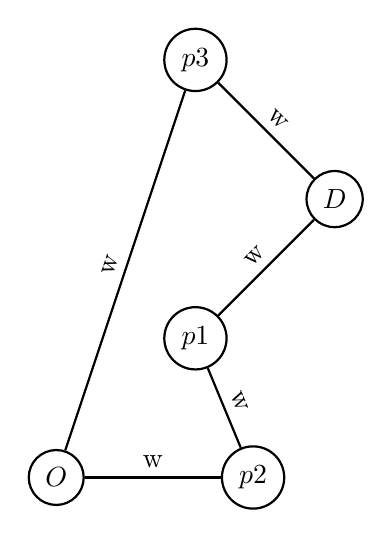
\begin{tikzpicture}[node distance={25mm}, thick, main/.style = {draw, circle}]
            \node[main] (1) {$O$};
            \node[main] (3) [above right of=1] {$p1$};
            \node[main] (2) [right of=1] {$p2$};
            \node[main] (4) [above right of=3] {$D$};
            \node[main] (5) [above left of=4] {$p3$};
            \draw (1) -- node[midway, above, sloped]{w} (2);
            \draw (3) -- node[midway, above, sloped]{w} (4);
            \draw (4) -- node[midway, above, sloped]{w} (5);
            \draw (5) -- node[midway, above, sloped]{w} (1);
            \draw (2) -- node[midway, above, sloped]{w} (3);
            \end{tikzpicture} 
            \caption{TSP without dummy node}
        \end{subfigure}%
        \hfill
        \begin{subfigure}[b]{0.45\textwidth}
            \centering
            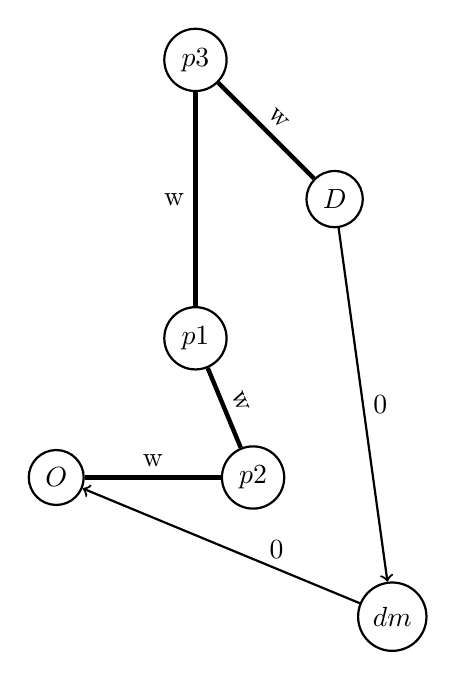
\begin{tikzpicture}[node distance={25mm}, thick, main/.style = {draw, circle}]
        
            \node[main] (1) {$O$};
            \node[main] (3) [above right of=1] {$p1$};
            \node[main] (2) [right of=1] {$p2$};
            \node[main] (4) [above right of=3] {$D$};
            \node[main] (5) [above left of=4] {$p3$};
            \node[main] (6) [below right of=2]{$dm$};
        
            \draw[ultra thick] (1) -- node[midway, above, sloped]{w} (2);
            \draw[ultra thick] (3) -- node[midway, left]{w} (5);
            \draw[ultra thick] (4) -- node[midway, above, sloped]{w} (5);
            \draw[ultra thick] (2) -- node[midway, above, sloped]{w} (3);
            \draw[->] (4) -- node[midway, right]{0} (6);
            \draw[->] (6) -- node[midway, above, pos=0.3]{0} (1);
            
            \end{tikzpicture}
            \caption{TSP with dummy node}
        \end{subfigure}
        \hfill \
        
        \caption{Adaptation to the TSP}
        \label{fig:tspadapt}
    \end{figure}
    
    \subsection{Held-Karp Algorithm} \label{heldkarp}
    The \textit{Held-Karp Algorithm} is an algorithm that solves the TSP using dynamic programming. This algorithm has a better time complexity comparing to the brute force solution, since it presents a $O(n^2 2^n)$ time complexity, which becomes better after some nodes. \cite{heldmankarp} However, we can verify that it still is exponential which doesn't make it a great solution, particularly if we have a large quantity of nodes.

    \begin{table}[h]
        \begin{center}
         \begin{tabular}{||c c c||} 
         \hline
         Points of Interest & Brute Force & Dynamic Programming \\ [0.5ex] 
         \hline\hline
         1 & 1 & 2 \\ 
         \hline
         2 & 2 & 16  \\
         \hline
         ... & ... & ... \\
         \hline
         6 & 720 & 2304 \\
         \hline
         7 & 5040 & 6272 \\
         \hline
         ... & ... & ... \\
         \hline
         17 & 355687428096000 & 37879808\\
         \hline
         18 & 6402373705728000 & 84934656 \\
         \hline
         19 & 121645100408832000 & 189267968 \\[1ex]
         \hline
        \end{tabular}
        \end{center}
        \captionof{table}{Brute force VS dynamic programming time complexity}
        \label{fig:bfdp}
    \end{table}
    
    \pagebreak
    
    \subsection{Heuristics} \label{heuristics}
    
    There are some heuristics that minimize the time complexity of the problem with very good approximations of the optimal solution. 
    
    \subsubsection{Nearest neighbour}
    
    This heuristic applies some sort of a greedy methodology and tries to find the best route by always choosing the next point in the tour to be the closest one, by starting in the $O$ node. Since we just want to approximate the best tour so that after we can apply other path finding algorithms, we'll just use the geographic distance between the nodes.
    
    \begin{algorithm}
    	\caption{Nearest neighbour} 
	    \begin{algorithmic}[1]
		
		\State $tour \leftarrow \{O\}$
        \State $last \leftarrow O$ 
        
		\While{
		    $poi$ not empty
		}
		    \State $minDist \leftarrow \inf$
		    \State $next \leftarrow nil$
		    \For{\textbf{each} $node \in poi$}
                \If{$dist(last, node) < minDist$}
                    \State $minDist \leftarrow dist(last, node)$
                    \State $next \leftarrow node$
                \EndIf
		    \EndFor
		    \State $push(tour, next)$
		    \State $last \leftarrow next$
		    \State $poi \leftarrow poi \setminus \{next\}$
		\EndWhile

        \State $push(tour, D)$
		
	    \end{algorithmic} 
	\end{algorithm}
    
    \pagebreak

    
    \subsubsection{Minimum Spanning Trees}
    
    Another possible heuristic is based on using minimum spanning trees. This technique usually finds a result - in this case the distance - $15\%$ to $20\%$ above the optimal solution, which in many applications is enough. This method is based on finding a minimum spanning tree and visiting the resulting tree with a depth first search. \cite{skienna1}. However, in our case, the graph has directed edges, because of the dummy node, so we can't use the strategy described in Figure \ref{fig:tspadapt} with this heuristic. We can however approximate and find a minimum spanning tree, leaving out the destination node, adding it at the end of the result, as done on the approach for the nearest neighbour solution.
    
    
    \begin{figure}[h]
        \hfill
        \begin{subfigure}[b]{0.45\textwidth}

            \centering
            \begin{tikzpicture}[node distance={25mm}, thick, main/.style = {draw, circle}]
        
            \node[main] (1) {$O$};
            \node[main] (3) [above right of=1] {$p1$};
            \node[main] (2) [right of=1] {$p2$};
            \node[main] (4) [above left of=4] {$p3$};

            \draw (1) -- node[midway, above, sloped]{$w_1$} (2);
            \draw (1) -- node[midway, above, sloped]{$w_2$} (3);
            \draw (3) -- node[midway, right]{$w_3$} (4);



            \end{tikzpicture}
            \caption{Possible Minimum Spanning Tree}

        \end{subfigure}%
        \hfill
        \begin{subfigure}[b]{0.45\textwidth}
            \centering
            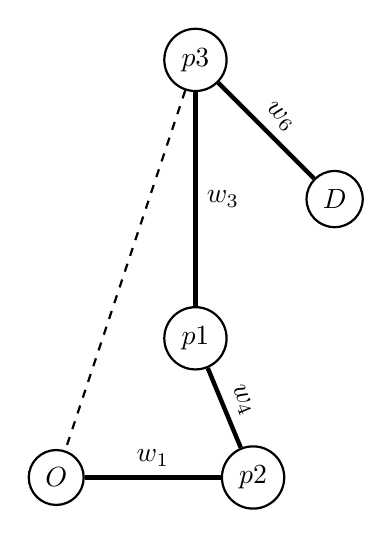
\begin{tikzpicture}[node distance={25mm}, thick, main/.style = {draw, circle}]
        
            \node[main] (1) {$O$};
            \node[main] (3) [above right of=1] {$p1$};
            \node[main] (2) [right of=1] {$p2$};
            \node[main] (4) [above right of=3] {$D$};
            \node[main] (5) [above left of=4] {$p3$};
        
            \draw[ultra thick] (1) -- node[midway, above, sloped]{$w_1$} (2);
            \draw[ultra thick] (3) -- node[midway, right]{$w_3$} (5);
            \draw[ultra thick] (4) -- node[midway, above, sloped]{$w_6$} (5);
            \draw[ultra thick] (2) -- node[midway, above, sloped]{$w_4$} (3);
            \draw[dashed] (5) -- (1);
            
            \end{tikzpicture}
            \caption{MST after BFS visit, adding D after the last node of the cycle}
        \end{subfigure}
        \hfill \vspace{0.1mm}
        \\ \\ \\
        \centering
        \begin{subfigure}[b]{0.45\textwidth}
            \centering
            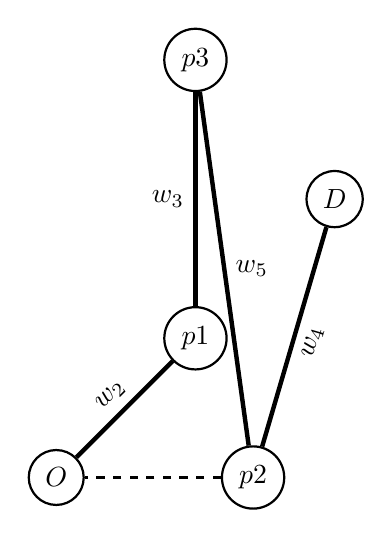
\begin{tikzpicture}[node distance={25mm}, thick, main/.style = {draw, circle}]
        
            \node[main] (1) {$O$};
            \node[main] (3) [above right of=1] {$p1$};
            \node[main] (2) [right of=1] {$p2$};
            \node[main] (4) [above right of=3] {$D$};
            \node[main] (5) [above left of=4] {$p3$};
        
            \draw[ultra thick] (1) -- node[midway, above, sloped]{$w_2$} (3);
            \draw[ultra thick] (3) -- node[midway, left]{$w_3$} (5);
            \draw[ultra thick] (2) -- node[midway, right]{$w_5$} (5);
            \draw[ultra thick] (2) -- node[midway, below, sloped]{$w_4$} (4);
            \draw[dashed] (2) -- (1);
            
            \end{tikzpicture}
            \caption{Another possible approximation, visiting in a different order}
        \end{subfigure}

        \caption{TSP with minimum spanning tree heuristic}
        \label{fig:tspmst}
    \end{figure}
    
    \pagebreak
    
    This heuristic can be applied with the following algorithm:
    
      \begin{algorithm}
    	\caption{TSP approximated using MST's} 
	    \begin{algorithmic}[1]
	    
	    \Function{$dfsVisit$}{$tour, current$}
            \State $push(tour, current)$
	        \For{each next in current}
                \State $visit(tour, next)$
    	    \EndFor
	    \EndFunction

	    \State $tour \leftarrow \{\}$
        \State $tree \leftarrow generateMst(O) \ // \ Either\ Kruskal's\ or\ Prim's\ algorithm,\ with\ O\ as\ root$ 
        \State $dfsVisit(tour, O)$
        \State $push(tour, D)$
		
	    \end{algorithmic} 
	\end{algorithm}
    
     \subsection{Defined Solution} \label{solution}
    
    As exposed, this problem has several solutions. However, all of them accuse a problem: where one lacks time and memory complexity, the other lacks solution accuracy relative to the best solution. As such, a way to minimize this problem is to use the solutions where they really do thrive.
    
    For that, one can use a dynamic programming approach for a small number of POI, as there is no need to compromise the result when the time and memory complexities are still small. As that number grows and the complexity becomes harder and harder to handle, a switch to either of the presented heuristics can be made. With this in mind, the compromise between complexity and the best solution is reduced and a better algorithm is presented.
    
    \chapter{Use Cases} \label{application}
     
    It is very difficult to find parking spots when traveling around the city and the solution to this problem is the basis for a mobile app that would help people select the best trip around a city and find parking lots near their desired locations. However, this project has a serious limitation: it is currently impossible to have all of the data needed to have a correct output. One of the most important data entries that is not easy to obtain is the park availability, since there is no service that provides that information. The solution to that problem is to allow the users to cooperate and share data with everyone, meaning that in parks that lack that information, the users would provide status on the park upon reaching there.
    
    \section{Actors}
    
    The applicability of this project is based on user cooperation and shared information, but an admin is also needed.
        
    \begin{enumerate}
        \item \textbf{User} - The application is centralized on the user. It will be him who will use the application to travel around the city and choose parameters to have a customized trip. It will be also the user who'll make it possible to have relatively updated information concerning a park's current capacity.
        \item \textbf{Admin} - The admin account has the ability to manage available parking spots and edit the map for unavailable streets, for example, adding or removing information to/from the map. 
    \end{enumerate}
    
    \section{Project Functionalities}
    
    This project will run in a terminal interface where the user can input the data previously stated. The user will choose the starting and destination points as well as the points of interest before reaching the destination. He will also type in the terminal the importance factors of the walking distance and parking price to better serve the user when choosing a park. Since the parks are affected by availability, it would be interesting to simulate users concurrency, trying to access parks at the same time. After the result is calculated, an animation will be displayed on a graph, showing the trajectory that the user should take.
    
    \pagebreak
     
    \chapter{Main Considerations and Preliminary Analysis} % 
    
    The problem at hand, "Looking for a parking place", was identified as being interesting, challenging and quite pertinent. The purpose of this report was to research and identify the problem and the algorithms needed to reach a solution.
    
    In order to better understand and quickly approach the problem, the group performed an analysis of a real world application of graphs in mapping systems, \textit{OpenStreetMap}. This helped understand how streets and parking lots are represented in a graph, resulting in a better formalization of the input data needed. Next followed the discussion of the various steps to solve the problem and the identification of a 'Travelling Salesman'-like problem.
    
    As such, the solution was split in three steps (Section \ref{analysis}): 
    \begin{enumerate}
        \item Finding the best parking spot, using Dijkstra's shortest path algorithm and filtering down the candidates (Subsection \ref{selectpark}). 
        \item Finding the shortest path to such candidate/s, using the A* Algorithm (Subsection \ref{selectpath}) using an heuristic as defined in subsection \ref{aheuristic}.
        \item Solving the 'Travelling Salesman'-like problem in finding the or an approximation of the best path to travel through all points of interest before reaching the destination (Section \ref{tspa}) which, by itself, also requires multiple steps:
        \begin{enumerate}
            \item Adapting the problem to a Travelling Salesman problem as explained in section \ref{tspa} and in Figure \ref{fig:tspadapt}.
            \item Solving this adaptation either by using the Held-Karp Algorithm (Subsection \ref{heldkarp}) or by using either heuristics referenced in subsection \ref{heuristics}, \textit{Nearest Neighbour} and \textit{Minimum Spanning Trees}.
        \end{enumerate}
    \end{enumerate}
    
    One of the main goals of this solution was to balance time complexity and accuracy, as it represents a real-life application that needs good and relatively fast results \ref{application}.
    
    Nevertheless, some issues may need to be addressed such as the work-around used to circumvent the impossibility of using directed graphs with the \textit{Minimum Spanning Trees} heuristic (subsection \ref{heuristics}) which can worsen its accuracy. In addition, finding the perfect compromise between complexity and accuracy (Subsection \ref{solution}), in choosing which algorithms to use in the Travelling Salesman Adaptation, can become hard as the line between what is considered a low or high amount of points of interest can be blurry.
    
    Despite these issues, the break down of the problem assigned to the group allowed a more organized, thought-out and coordinated solution which will surely reduce the complexity and time needed to fulfill the goals of the project.
    
    \pagebreak
    
    \chapter{Contributions}
    
    All members of the group worked together to come up with this solution and its report. The effort was distributed evenly and, as such, each member has a 33.3\% contribution rate. 
    
    All members were equally involved in the formalization of the problem and definition of the input data, output data, restrictions and objective functions.
    
    André Moreira took a deeper approach to the TSP problem, formalizing its heuristics and possible algorithms.
    
    Nuno Alves formalized the Dijkstra solution and its intricacies, as well as the use cases and main considerations to take from this project.
    
    Nuno Costa approached the graph connectivity problem and the A* adaptation for the path problem.
    
    It must be noted, however, that even though all members were involved in distinct parts in a deeper manner, the cooperation in all aspects and chapters of this report existed and was maintained throughout. 
    
    \pagebreak
    
    \printbibliography
    
\end{document}
